\subsection{Frozen-feature validation}\label{app:frozen-validation}

The five-million-update comparison tests the theorem against executed GD at
every update. At bandwidths $1/32,1/16,1/8,1/4$, the smallest ratios of
predicted lower error to actual error are respectively
$0.9632,0.7544,0.8275,0.8471$. At the final update they are
$0.9985,0.9516,0.9058,0.9308$. The maximum apparent lower-bound violation is
$1.1\times10^{-15}$; the independently evaluated exact-spectrum error differs
from executed GD by at most $2.9\times10^{-14}$. Refining the center quadrature
changes the predicted error by at most $9.6\times10^{-11}$. These checks
support the plotted floating-point calculation over the tested horizons and
geometries.

\begin{figure}[t]
\centering
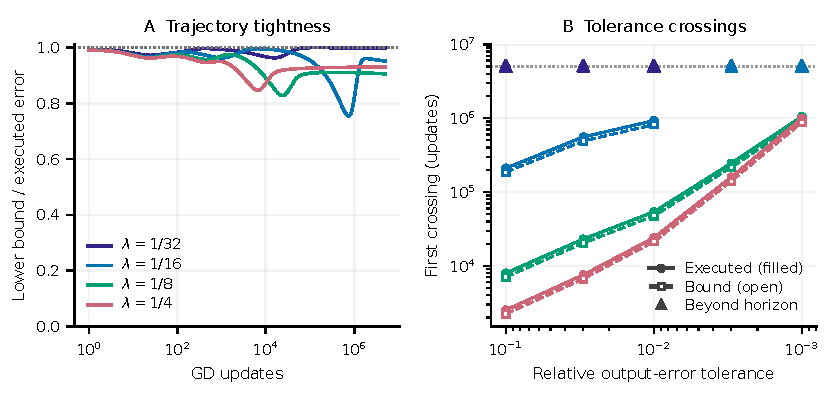
\includegraphics[width=\linewidth]{output/diagnostics/section34_long_horizon/main_5m/bound_diagnostics/bound_diagnostics.pdf}
\caption{\textbf{Theorem validation over five million updates.}
Left: predicted lower error divided by executed GD error; one denotes
equality. Display curves use a mixed logarithmic/linear grid, while the
reported extrema inspect every update. Right: first crossings of several
output-error tolerances, with necessary times from the theorem shown open
and executed crossings filled. Triangles indicate no crossing within the
horizon, not estimated crossing times. Among uncensored comparisons,
necessary times are $88.35$--$88.42\%$ of executed times. No tolerance defines
circuit usability in this experiment.}
\label{fig:slope-bound-tightness}
\end{figure}

Attainability and optimization are separate. At $\lambda=1/32$, a directly
fitted readout has dense-grid relative error $6.24\times10^{-10}$, whereas
GD retains error $0.210$ after five million updates. At $\lambda=1/4$, the
same GD protocol reaches $3.88\times10^{-4}$. The direct fits retain singular
values above $10^{-12}$ times the largest singular value, and the very
accurate small-slope fit has readout $\ell_1$ norm
about $7.5\times10^3$. It witnesses attainability without claiming that the
corresponding coefficients are easy to learn.

The slow error has the expected frequency content. Projecting the executed
residual onto the three orthogonal target harmonics shows that
$\sin(14\pi x)$ accounts for $95.41\%$ of remaining residual energy at
$\lambda=1/32$ after five million updates. At its frequency, the feature
multiplier is $M_\gamma(14\pi)=0.001463$ for $\lambda=1/32$ and $0.799774$
for $1/4$. These values describe feature smoothing, not eigenvalue ratios.
The finite-kernel theorem accounts for the geometry connecting smoothing to
GD rates. At larger bandwidths, the late residual lies predominantly outside
the three input harmonics, illustrating why the full finite kernel remains
relevant even for a target with only three frequencies.

\begin{figure}[t]
\centering
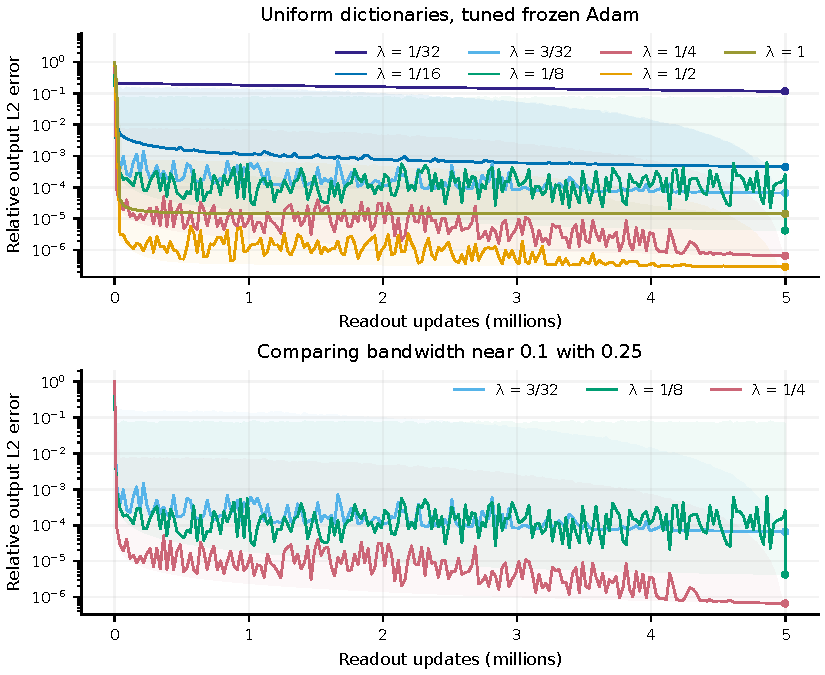
\includegraphics[width=\linewidth]{output/diagnostics/section34_long_horizon/main_5m/uniform_access/uniform_adam_trajectories.pdf}
\caption{\textbf{Frozen Adam under the same five-million-update budget.}
Each curve uses one complete recipe chosen by final validation error from
the shared expanded search. Lines aggregate compact bin medians into 200
display intervals; shading preserves every within-bin extremum, and dots
mark exact endpoint errors. The lower panel isolates $\lambda=3/32,1/8,1/4$, whose
final dense-grid errors are $6.63\times10^{-5}$, $4.26\times10^{-6}$, and
$6.62\times10^{-7}$. Thus $\lambda=3/32\approx0.094$ leaves about 100 times
the error of $1/4$, while $1/8$ leaves 6.44 times its error.
These are empirical Adam trajectories, not evaluations
of the GD bound.}
\label{fig:slope-frozen-adam}
\end{figure}

The three recipes highlighted in Figure~\ref{fig:slope-frozen-adam} are
cosine Adam at $0.002$, constant Adam at $0.001$, and cosine Adam at $10^{-4}$,
respectively. The constant-rate trajectory remains noisy, so its final
error is not a sustained level. The full sweep is not monotone: $\lambda=1$ is worse than
$1/2$, consistent with the target-dependent tradeoff in the construction.
The reference bandwidth $1/4$ was fixed before this comparison. It is a
useful supplied geometry, not a fitted universal optimum or a threshold
that applies to heterogeneous learned features.
